\documentclass{article}

\usepackage[utf8]{inputenc}
\usepackage{graphicx}
 \usepackage{hyperref}

\title{A Report on Fake News Detector}

\author{2018-1-60-212, 2018-1-60-213, 2018-1-60-215, 2018-1-60-165}
\date{January 2022}

\begin{document}

\maketitle

\section{Introduction:}
  Fake news is a type of news which are generated intentionally to misguide the readers. It is a type of propaganda which is published in the form of genuine news. Fake news is spread through traditional news media and social media. The spreading of fake news has been a problem for a long time. With the introduction of social media, the spread of fake news has continued to increase, and it has become too difficult to distinguish between true news and fake news. The spread of fake news is a matter of concern as it manipulates the public opinions. The wide spread of fake news can have a huge negative impact on individuals and society. We developed a model which accurately determines whether an article is fake or not using machine learning algorithm logistics regression and NLP techniques.
   
\subsection{Objectives:}
    Our main objective of the project is to identify whether some news is real or fake from a dataset based on a list of real and fake news compiled from Kaggle. Moreover, some other objectives of this project are:
    \begin{itemize}
    \item	Taking the help of linguistic cues to develop a machine learning based model for accurately determining whether the news from the dataset is fake or real.
    \item To generate high accuracy in order to determine whether some news is fake or not.
\end{itemize}
   


   \subsection{Motivation:}
   The project we were tasked to complete was to be based on machine learning. As we were browsing through the internet brainstorming ideas on a good topic, we came across a lot of misleading websites which not only wasted our precious time but was an irritating experience as well. Upon some investigation, we found that fake news is harming the general people in many ways possible. The extensive spread of fake news is continuing to create a serious negative impact on individuals and society. It has taken down the authenticity of the news ecosystem as it is even more widely spread on social media than most popular authentic news portals. It is becoming one of the biggest problems which can change opinions and influence decisions and interrupt the way of people responding to real news. We aim to develop a model using machine learning algorithms to determine whether some news is fake or real.
   
    \subsection{Existing Works:}
    Several algorithms were used before in order to create this project. Various papers were published as well. Various approaches were taken as well. We present two of the works we studied on before engaging on our project:\break\break
    \textbf{Fake News Detection Using Logistic Regression and Boolean crowdsourcing algorithms:}
 Social network sites (SNSs) have revolutionized the way in which information is spread by allowing users to freely share content. Therefore, SNSs are also increasingly used as vectors for the diffusion of misinformation and hoaxes. In this experiment, the performance of the logistic regression and Boolean crowdsourcing algorithms via a set of experimental datasets was characterized. In general, only via a laborious process of manual post inspection, the results indicated how much investment was needed in manual labeling, to reap the benefits of automated classification. The second set of experiments measured how much information learning is needed to transfer from one set of pages to another[1].\break\break
\textbf{Fake News Detection Using Knowledge Verification and Natural Language Processing:} The main purpose was to explore the ‘fake news’ as a disinformation implement. They tried to establish a new solid definition of ‘fake news’ in terms of comparative bias and factual accuracy. For detecting fake news in the datasheet, NLP model was used as a proposed solution. This classification model consists of NLP features combined with some knowledge verification to maintain the reliability of the source. For textual input, NLP features like stop-words percentage, title length, readability and sentiment score had been used for analysis. On the other hand, knowledge verification features id the answer to the question whether the title look like more than one sources or whether the title seems to be based on facts or opinion[2].

 \subsection{Necessity:}
   News are the source of knowledge and source of power for a lot of people around the world. Not everyone engages in watching televisions or have the luxury to own one. However, in the era of internet, news is easier to search and read. That is why news should be filtered and an approach should be made so that the real news is to be reached to the general people. Fake news can change the opinion of a person towards something, can create imbalance and hate, can manipulate people into doing wrongdoings. A great example of fake news is the US election of 2016 where Donald Trump hired a data processing company called ‘Cambridge Analytica’ to advertise his election campaign. However, his hidden motive was to manipulate the general people into voting him and create hate towards his opposing party. Therefore, fake news detection is a necessity on the slowly developing field of the news platform on the internet.
   
    \section{Methodology:}
  We have used different kinds of algorithm in order to train and test our dataset. In different algorithm we have find different kinds of algorithm showing different kinds of result. Every algorithm has different kind of approach in order to train dataset and because of that we have got different accuracy for same dataset. We have used:
\begin{itemize}
    \item Logistic Regression
    \item Multinomial Naïve Bayes
    \item Decision Tree Classifier
    \item Random Forest Classifier
\end{itemize}
   
   \section{Implementation: }
 \subsection{Data collection:}
 For conducting our project fake news detector, we collected our train dataset from Kaggle. Train dataset link is - \url{https://www.kaggle.com/c/fake-news/data}\break
Train dataset has some following attributes:
\begin{itemize}
    \item id: distinctive id for each news article
    \item title: news article’s title
    \item author: news article’s author
    \item text: news article’s text. It might be empty
    \item Label: indication false and real news. Here,
    \begin{itemize}
    \item 1 is indicating to False News
    \item 0 is indicating to Real News
    \end{itemize}
\end{itemize}
   \subsection{Data processing:}
   In order to train our train our dataset we must process our data in the dataset. For processing our data, we must do follow some steps:
   \begin{itemize}
    \item id in our dataset is not necessary in order to train our dataset. So, we have dropped this column from our dataset.
    \item In the dataset, there are some null values, we have replaced the null values with empty strings.
    \item In order to train our dataset, we have used news’s author’s name and the news’s title. We joined author’s name and news title together and labeled that as content. 
    \item We only kept letters in the content and delete all the other things.
    \item We changed all the letters into small letters.
    \item Then we delete unnecessary words like  'me', 'i', 'my', 'myself', 'we', 'our', 'ours', 'ourselves', 'you', "you're", "you've", "you'll", "you'd", 'your', 'yours', 'yourself', 'yourselves', 'he', 'him', 'his', 'himself', 'she', "she's", 'her', 'hers', 'herself', 'it', "it's", 'its', 'itself', 'they', 'them', 'their', 'theirs', 'themselves', 'what', 'which', 'who', 'whom', 'this', 'that', "that'll", 'these', 'those', 'am', 'is', 'are', 'was', 'were', 'be', 'been', 'being', 'have', 'has', 'had', 'having', 'do', 'does', 'did', 'doing', 'a', 'an', 'the', 'and', 'but', 'if', 'or', 'because', 'as', 'until', 'while', 'of', 'at', 'by', 'for', 'with', 'about', 'against', 'between', 'into', 'through', 'during', 'before', 'after', 'above', 'below', 'to', 'from', 'up', 'down', 'in', 'out', 'on', 'off', 'over', 'under', 'again', 'further', 'then', 'once', 'here', 'there', 'when', 'where', 'why', 'how', 'all', 'any', 'both', 'each', 'few', 'more', 'most', 'other', 'some', 'such', 'no', 'nor', 'not', 'only', 'own', 'same', 'so', 'than', 'too', 'very', 's', 't', 'can', 'will', 'just', 'don', "don't", 'should', "should've", 'now', 'd', 'll', 'm', 'o', 're', 've', 'y', 'ain', 'aren', "aren't", 'couldn', "couldn't", 'didn', "didn't", 'doesn', "doesn't", 'hadn', "hadn't", 'hasn', "hasn't", 'haven', "haven't", 'isn', "isn't", 'ma', 'mightn', "mightn't", 'mustn', "mustn't", 'needn', "needn't", 'shan', "shan't", 'shouldn', "shouldn't", 'wasn', "wasn't", 'weren', "weren't", 'won', "won't", 'wouldn', "wouldn't" etc. from our content.
    \end{itemize}\break
    \begin{figure}[!h]
    \centering
    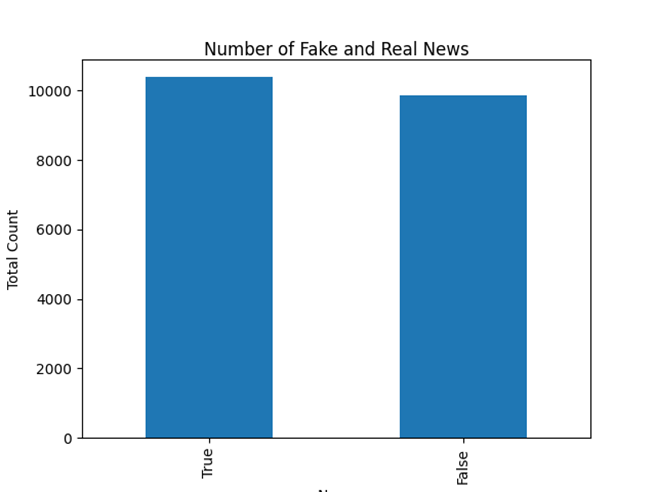
\includegraphics[width=0.8\textwidth]{image1.png}
    \caption{Total Real and Fake News}
    \label{fig:label}
    \end{figure}
    In the Figure 1, we can see that the total number of real and false news in our dataset in a bar chart.\break
    \begin{figure}[!h]
    \centering
    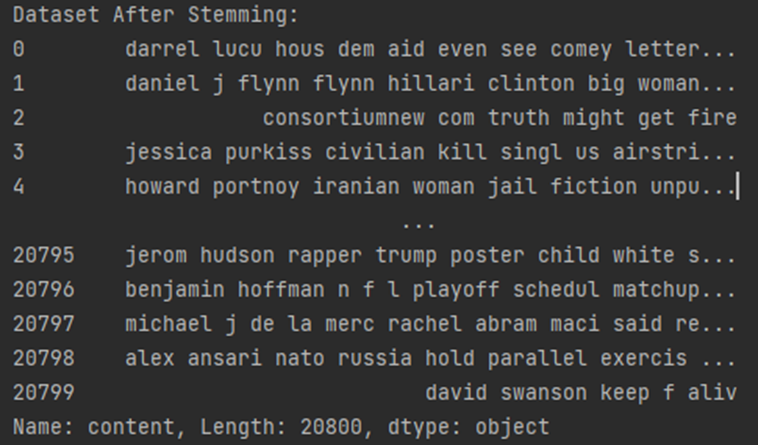
\includegraphics[width=0.8\textwidth]{image2.png}
    \caption{Dataset After Stemming Process}
    \label{fig:label}
    \end{figure}
    \break
    In the figure 2, we can see the dataset after the stemming process. In the stemming process we only kept the letters and delete all the numerical data, commas and many more things. Then we convert all the letters into small letters. Then we have deleted all the unnecessary words from the dataset and finally by joining all the words we have prepared our dataset.\break
    \begin{figure}[!h]
    \centering
    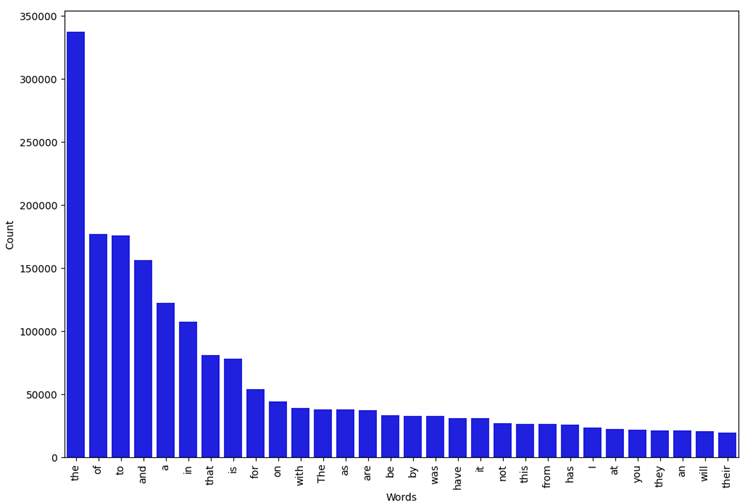
\includegraphics[width=0.8\textwidth]{image3.png}
    \caption{Word Count of False News}
    \label{fig:label}
    \end{figure}\break
    In the figure 3, we can see the words count of the false news from the dataset. This bar chart represents the chain of most used of words that were used in the false news. Since there were a lot of words, so we are only showing the first fifty most used words in the chart from the dataset.\break
    \begin{figure}[!h]
    \centering
    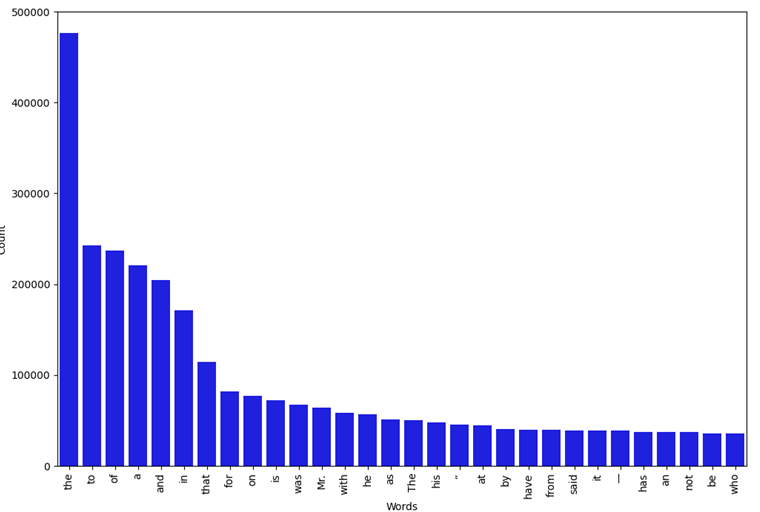
\includegraphics[width=0.8\textwidth]{image4.png}
    \caption{Word Count of Real News}
    \label{fig:label}
    \end{figure}\break
    In the figure 4, we can see the words count of the real news from the dataset. This bar chart represents the chain of most used of words that were used in the real news. Since there were a lot of words, so we are only showing the first fifty most used words in the chart from the dataset.
    \break
    \begin{figure}[!h]
    \centering
    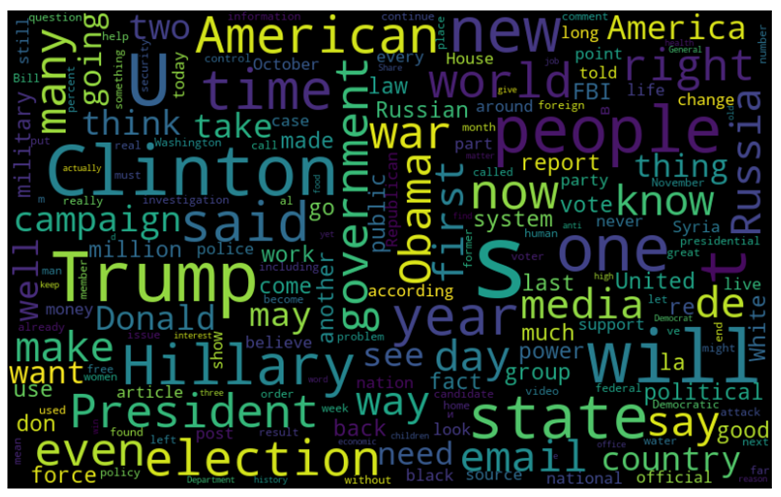
\includegraphics[width=0.8\textwidth]{image5.png}
    \caption{Word Count of Real News}
    \label{fig:label}
    \end{figure}\break
    In the figure 5, we can see the word cloud of false news in a visualization method.  Here we can see the most used words in a false news from the dataset. 
    \break
    \begin{figure}[!h]
    \centering
    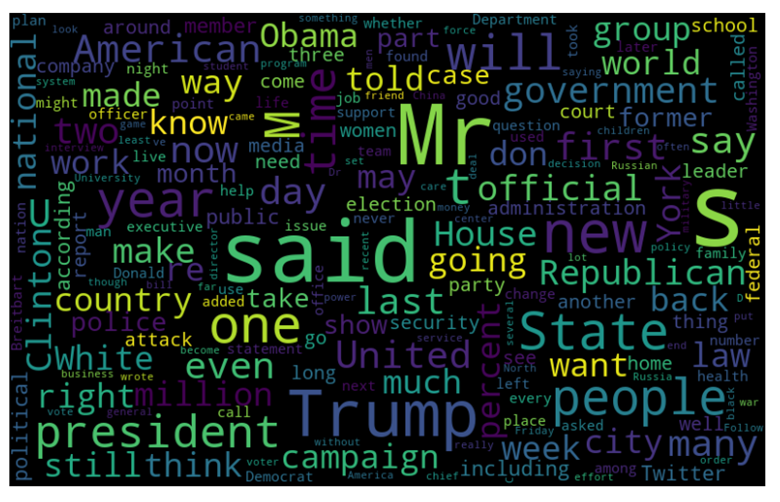
\includegraphics[width=0.8\textwidth]{image6.png}
    \caption{Word Count of Real News}
    \label{fig:label}
    \end{figure}\break
    In the figure 6, we can see the word cloud of real news in a visualization method.  Here we can see the most used words in a real news from the dataset.
    \break
    
    
    \subsection{Model Development:}
   For developing our model, we have used python interpreter and we have used IDE- Pycharm Community Edition. We have used some library functions such as ‘numpy’, ‘pandas’, ‘re’, ‘matplotlib’, ‘seaborn’, ‘nltk’, ‘itertools’, ‘sklearn’, ‘wordcloud’.
    
    
    \subsection{Results:}
    We have tested several methods and algorithm to train and test our dataset. We get excellent results from those methods and algorithm. The tested algorithm results are given below:
        \subsubsection{CountVectorizer \& Logistic Regression:}
    
    \begin{figure}[!h]
    \centering
    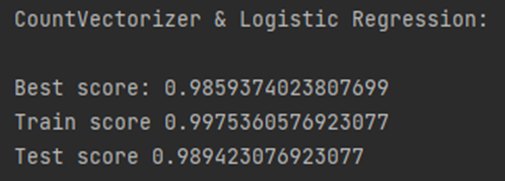
\includegraphics[width=0.8\textwidth]{image7.png}
    \caption{Accuracy Score using CountVectorizer \& Logistic Regression}
    \label{fig:label}
    \end{figure}\break
In the figure 7, we can see that using countvectorizer and logistic regression we are getting these scores. We are seeing that the train dataset score is 99 \% which is showing a great training score. The test dataset score is almost near to 99 \% which is a great result for the dataset. Confusion matrix for this method is given below: \break
   \begin{figure}[!h]
    \centering
    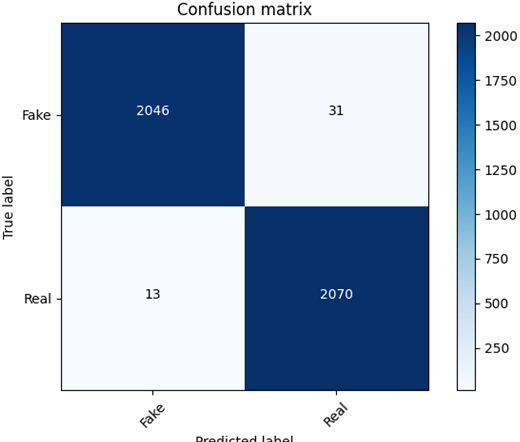
\includegraphics[width=0.8\textwidth]{image8.png}
    \caption{Confusion Matrix using CountVectorizer \& Logistic Regression}
    \label{fig:label}
    \end{figure}\break
    In the figure 8, we can see the confusion matrix, which was built by using count vectorizer method and logistic regression algorithm and it shows how much accurate result is giving this model on the dataset.
    \subsubsection{TfidfVectorize \& Logistic Regression}
    \begin{figure}[!h]
    \centering
    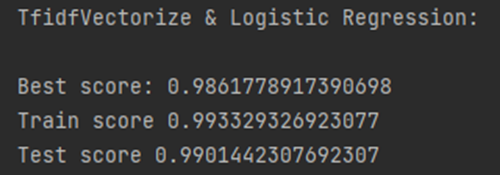
\includegraphics[width=0.8\textwidth]{image9.png}
    \caption{Accuracy Score using CountVectorizer \& Logistic Regression}
    \label{fig:label}
    \end{figure}\break
    In figure 9 we can see the train and test dataset scores both are 99\% and the best score for this method is showing 98\%.  Confusion matrix for this model is given below:\break
    \begin{figure}[!h]
    \centering
    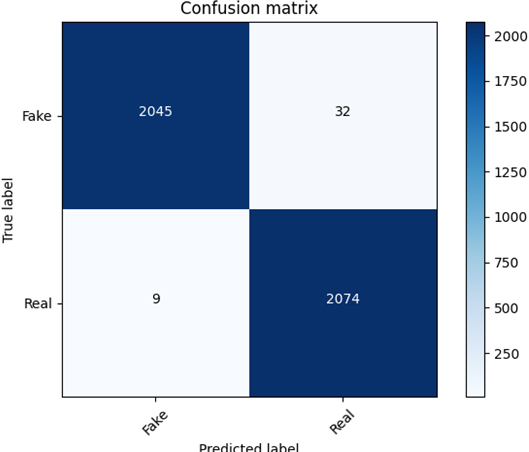
\includegraphics[width=0.8\textwidth]{image10.png}
    \caption{Confusion Matrix using TfidfVectorize \& Logistic Regression}
    \label{fig:label}
    \end{figure}\break
    In the figure 10, we can see the confusion matrix, which was built by using TfidVectorizer method and logistic regression algorithm and it shows how much accurate result is giving this model on the dataset.
    \subsubsection{CountVectorizer \& MultinomialNB}
     \begin{figure}[!h]
    \centering
    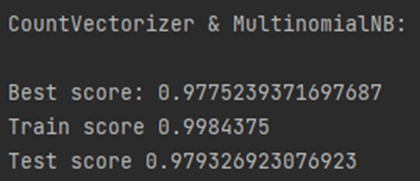
\includegraphics[width=0.8\textwidth]{image11.png}
    \caption{Accuracy Score using CountVectorizer \& MultinomialNB}
    \label{fig:label}
    \end{figure}\break
    In the figure 11, we can see the train and test dataset accuracy score using multinomial naïve bayes algorithm. The train dataset is showing 99\% score and the test dataset is showing 97\% score. For this algorithm we are getting 97\% accuracy for our dataset. Confusion matrix for this algorithm is given below:
    \break
    \begin{figure}[!h]
    \centering
    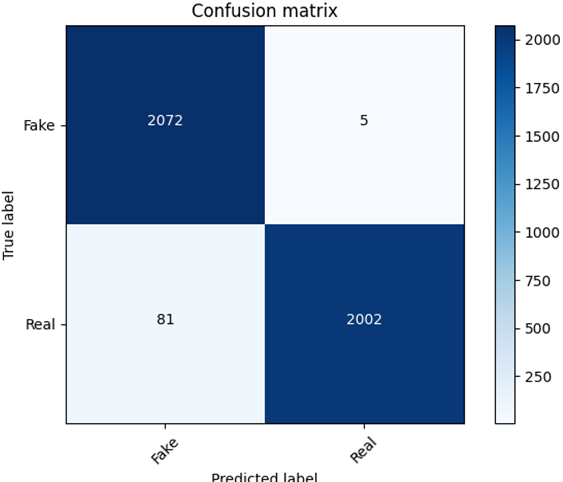
\includegraphics[width=0.8\textwidth]{image12.png}
    \caption{Accuracy Score using CountVectorizer \& MultinomialNB}
    \label{fig:label}
    \end{figure}\break
    In the figure 12, we can see the confusion matrix, which was built by using CountVectorizer method and MultinomialNB algorithm. Here we can see that the confusion matrix is showing excellent result in showing the correct result.
    \subsubsection{TfidfVectorizer \& MultinomialNB}
     \begin{figure}[!h]
    \centering
    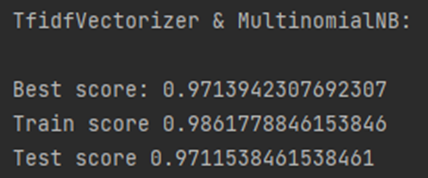
\includegraphics[width=0.8\textwidth]{image13.png}
    \caption{Accuracy Score using CountVectorizer \& MultinomialNB}
    \label{fig:label}
    \end{figure}\break
    In the figure 13, we can see that the in the TfidVectorizer method using multinomial naïve bayes algorithm we are getting 98\% accuracy score for the dataset which is used for training and 97\% accuracy score for the dataset which is for testing.  Best score for our train and test dataset we are getting 97\%. Confusion matrix for this method is given below:\break
    \begin{figure}[!h]
    \centering
    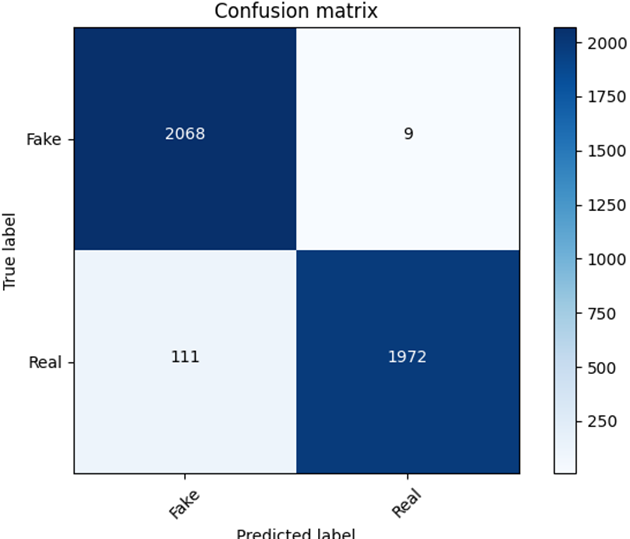
\includegraphics[width=0.8\textwidth]{image14.png}
    \caption{Confusion Matrix using TfidfVectorizer \& MultinomialNB}
    \label{fig:label}
    \end{figure}\break
    In the figure 14, we can see the confusion matrix, which was built by using TfidfVectorizer method and MultinomialNB algorithm. 
    
\subsubsection{Decision Tree Classifier}
     \begin{figure}[!h]
    \centering
    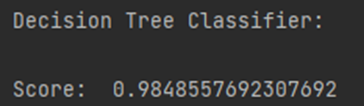
\includegraphics[width=0.8\textwidth]{image15.png}
    \caption{Confusion Matrix using TfidfVectorizer \& MultinomialNB}
    \label{fig:label}
    \end{figure}\break
    In the figure 15 we can see that using countvectorizer method along with tfidtransformer and applying logistic regression algorithm we are getting accuracy score for our dataset is 98\%. This is known as decision tree classifier accuracy score. Confusion matrix for decision tree classifier is given below: 
    \break
    \begin{figure}[!h]
    \centering
    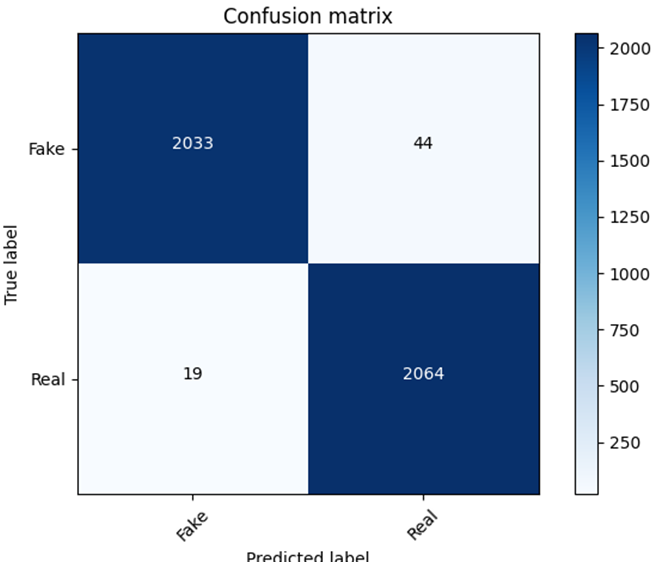
\includegraphics[width=0.8\textwidth]{image16.png}
    \caption{Confusion Matrix using CountVectorizer, TfidfTransformer \& Logistic Regression}
    \label{fig:label}
    \end{figure}\break
    In the figure 16, we can see the confusion matrix, which was built by using TfidfVectorizer method, TfidfTransformer method and MultinomialNB algorithm. Here we can see that the confusion matrix is showing excellent result in showing the correct result.
    
    \subsubsection{Random Forest Classifier}
     \begin{figure}[!h]
    \centering
    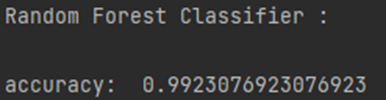
\includegraphics[width=0.8\textwidth]{image17.png}
    \caption{Accuracy Score using Random Forest Classifier}
    \label{fig:label}
    \end{figure}\break
    In the figure 17, we are seeing that using random forest classifier algorithm on our dataset we are getting 99\% accuracy result on our dataset. Confusion matrix for this model is given below:
    \break
    \begin{figure}[!h]
    \centering
    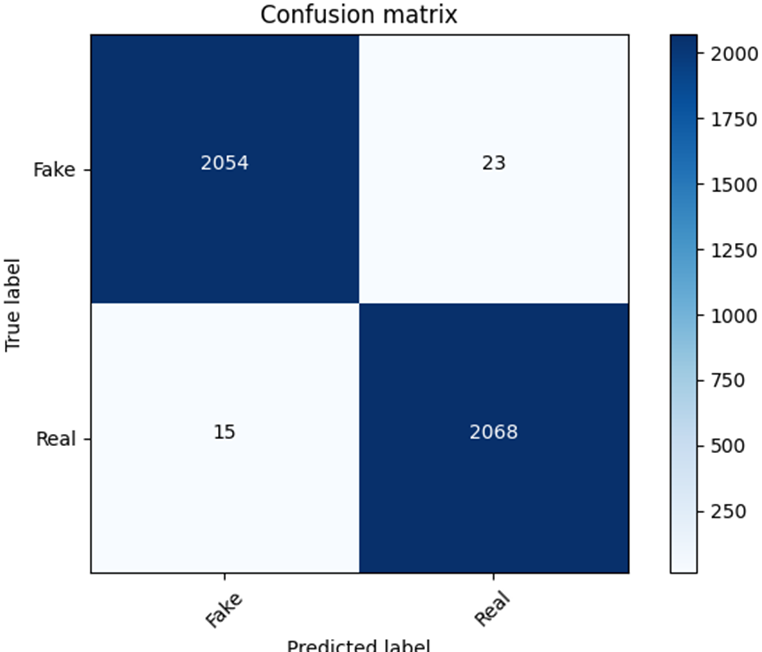
\includegraphics[width=0.8\textwidth]{image18.png}
    \caption{Confusion Matrix using CountVectorizer, TfidfTransformer \& RandomForestClassifier}
    \label{fig:label}
    \end{figure}\break
    In the figure 18, we can see the confusion matrix, which was built by using TfidfVectorizer method, TfidfTransformer method and RandomForestClassifier algorithm.
    
    \section{Conclusions:}
    The vast spreading of fake news can create a bad impact on people.  People are misled by fake news it is also the ultimate confusion. People with their naked eyes cannot distinguish between real news and fake news. And this is a real danger of fake news. We can predict news to be real or fake by using the power of machine learning and with this power, we can solve this problem.
    
       \subsection{Challenges:}
   In this project, we have used different kinds of algorithms. By using these algorithms, we can train and test our dataset and can find different kinds of results. But before using these algorithms we didn’t know which algorithm is good for our dataset and which one would give us the accurate result. So, this was our challenge for our project. We have used - Multinomial Naïve Bayes, Logistic Regression, Random Forest Classifier, Decision Tree Classifier.
       \subsection{Limitations:}
        In this project, we have used different kinds of algorithms. We have used - Multinomial Naïve Bayes, Logistic Regression, Random Forest Classifier, Decision Tree Classifier. By using these algorithms, we train, test, and preprocess our dataset for getting results. But if we change our dataset our algorithms will not give an accurate result. For different datasets, we need to train, test and pre-process the dataset for getting results again. And this is our limitation.
Fake news spread very rapidly and reaches on social media. Without collaborative access and compromising speed it's hard to study and design technological, computational, and combat business strategies. Normally, fake news is related to our emotions, ideological prejudices, exploiting our cognitive skills, so it's hard to identify. Also, detecting fake news by using computational methods is challenging. Lack of Susceptibility and public awareness are also hard to control fake news. Social media users fail to differentiate between legitimate news and false and fake news can easily reach a huge number of people in a short amount of time. 

          \subsection{Future Directions:}
        In this project, we have used different kinds of algorithms. We have used - Multinomial Naïve Bayes, Logistic Regression, Random Forest Classifier, Decision Tree Classifier. In the future, we will implement other algorithms of machine learning. We will try to find more accurate percentages than our current algorithms can do. We can use our system for new and for large number data set in the future. That will help us to understand the latency level and the computational speed in advance. In the future, we can also implement this same dataset for the different machine learning algorithms. For doing this we can compare which model or algorithm is better and outperformed.
    \section{Reference:}
        

[1]	E. Tacchini, G. Ballarin, M. L. della Vedova, S. Moret, and L. de Alfaro, “Some like it Hoax: Automated fake news detection in social networks,” in CEUR Workshop Proceedings, 2017, vol. 1960.\break\break
[2]	M. D. Ibrishimova and K. F. Li, “A machine learning approach to fake news detection using knowledge verification and natural language processing,” in Advances in Intelligent Systems and Computing, 2020, vol. 1035. doi: 10.1007/978-3-030-29035-1\_22.

        
   \end{document}
   
